\documentclass[a4paper]{article}
\usepackage[utf8]{inputenc}
\usepackage[T1]{fontenc}
\usepackage{times}
\usepackage[margin=3cm]{geometry}

% German
%\usepackage[ngerman]{babel}
% English
\usepackage[english]{babel}

\usepackage[round,authoryear]{natbib}
\usepackage{amsmath,amssymb,amsthm}
\usepackage[hyphens]{url}
\usepackage{graphicx}
\usepackage{booktabs}

\usepackage{tabularx} % ist das erlaubt?
\usepackage{float}


\usepackage{lipsum}

% German
%\newtheorem{definition}{Definition}
%\newtheorem{satz}{Satz}
% English
\newtheorem{definition}{Definition}
\newtheorem{theorem}{Theorem}

% FRAGEN
% zitat jedes einzelne mal angeben, zb bei Pung?
% was gehört alles zu seiten 10-12, auch references? 
% wie viele verwandte themen bei related work? dürfen es auch diese sein, die im paper schon diskutiert wurden? 

% TODO
% Addra zeiten in tabelle und generell vergleich 

\author{Carina Fehr}
\title{Seminar Report on Express: Lowering the Cost of Metadata-hiding Communication with Cryptographic Privacy}
\date{\today}

\begin{document}

\maketitle

\begin{abstract}
This report studies the reproducibility and performance of Express, a system designed for metadata-hiding communication. Using two servers, Express ensures cryptographic security against at most one malicious server and an arbitrary number of malicious clients. The paper presents new protocols that offer low communication overhead, regardless of the number of users, and improved computation costs using symmetric key cryptography. Compared to Pung and Riposte, two previous cryptographically secure systems, Express achieves increased message throughput while maintaining strong privacy guarantees. This makes Express an ideal application for communication with whistleblowers.
\end{abstract}

\section{Introduction}
\label{sec:intro}
In modern computer networks, secure communication is becoming increasingly crucial, given the growing capabilities of surveillance and metadata analysis. Although secure messaging apps like Signal and Threema, as well as Transport Layer Security (TLS), encrypt the content of sent messages, they do not protect metadata. It is possible to observe who sent and received messages, when and how often they communicated, and how much data they exchanged. This information is as sensitive as the messages themselves and should therefore not be leaked. However, it is challenging to keep all data hidden, as most internet-based communication services rely on some of the metadata to process messages. One option for hiding metadata would be to use a Tor browser or SecureDrop, but these are vulnerable to attacks by adversaries who control many network points.  Other existing systems for metadata-hiding either have too high communication cost to be practical, or they have low computation cost, but their security gets worse with every round of communication, also making them impractical.\\
Express \citep{Eskandarian2021} offers a new communication option that keeps metadata private while ensuring feasible costs and calculation times. Although two servers are required, Express can still run with one malicious server. 
The target audience for Express are whistleblowers. To receive messages, a journalist or anyone else who should receive information must register a mailbox with the two servers. The servers allocate storage for the physical mailbox and maintain a page table that maps it to a unique virtual address, adding an extra layer of protection. The journalist can transmit these addresses to the whistleblower. Now the whistleblower can upload a message into the mailbox as a second client. No one except the mailbox owner will know that a message has been sent into this mailbox. Mailbox owners have to check their mailboxes regularly. Express does not hide when a client read from a mailbox, therefore a pattern in the checking intervals could reveal information about the activity of this mailbox. Additionally, Express must implement the option of cover traffic.  This will ensure that whistleblowers cannot be accused of disclosing information simply for contacting an Express server. In section \ref{sec:whistleblowing}, we will discuss in more detail how express can be used to communicate with whistleblowers.\\
There are different types of attacks that Express must be resilient against.
As all clients can read from all mailboxes, Express must re-encrypt the mailboxes each time a read occurs, providing encryption that only the owner can decrypt. Otherwise, an attacker could find out which client wrote into which mailbox by reading and comparing the content of all mailboxes between every pair of writes. Another possible threat would be a malicious client targeting all mailboxes, trying to prevent honest clients to communicate with each other. They could overwrite all mailboxes with one message. Because the mailboxes can only hold one message at a time, any messages sent before this would be lost in a denial-of-service attack. The complete overview is divided between the two servers, which means that the servers alone cannot recognise an invalid message. A new auditing protocol is used to prevent such attacks. This auditing scheme runs with constant client side computations and reduces the costs for the client by 8$\times$ for an installation with one million registered mailboxes compared to previous work. In Chapter \ref{sec:relwork}, we provide a deeper insight into the performance and costs of Express and compare it with similar communication systems. However, a malicious client could still attack a single mailbox. In this case, the message would appear legitimate, and the server would be unable to detect or prevent the attack. Virtual addresses are used to prevent the original messages in the mailbox from being overwritten. The address range is so large that the probability of hitting a specific mailbox is negligible. We will explain in more detail in section \ref{sec:protecting} how express protects against these various attacks.

\section{Background}
\label{sec:background}
This section explains two key concepts that form the foundation of Express: cryptographic privacy and distributed point functions, also called DPFs. In section \ref{sec:private}, we will show how they can be used to achieve efficient metadata-hiding communication.

\subsection{Cryptographic privacy}
\label{subsec:first-background}
Cryptographic privacy is a mechanism that guarantees no information about communication metadata is leaked to an adversary. Even after observing many rounds of communication, a global adversary with the ability to observe all network traffic cannot determine which clients are communicating with each other or to which mailbox a message was written to. \\
An alternative mechanism is differential privacy. After several rounds of communication, systems based on differential privacy, such as Vuvuzela or Stadium, will lose security. Consistent observation will allow the adversary to learn something about underlying communication patterns, resulting in a loss of anonymity over time. Therefore, although differential privacy is faster and involves lower computational cost, cryptographic privacy is the preferred approach for frequently used applications where long-term security is essential, such as Express.  


\subsection{Distributed point function}
\label{subsec:DPF}
A DPF \citep{DPF2023} is a cryptographic algorithm. It splits a function $f$ into function shares that individually hide $f$. Two parties A and B hold function shares $f_A$ and $f_B$, such that for any input $x$ the output is $f_A(x) + f_B(x) = f_{i,m}(x)$. The secret point function $f_{i,m}(x)$ outputs $m$ at the point $x = i$ and $0$ everywhere else. It is possible to create more than two function shares, which then work according to the same system, i.e., they are also added together. The two or more parts of the function individually reveal nothing about the function, so neither the location $i$ nor the value $m$. DPFs provide a compressed secret-sharing of a secret vector with weight one. \\
Express splits the function into two parts, one for each of the servers. The point $i$ is the mailbox index, the value $m$ is the message. 
Because no server alone can reconstruct the full function, even a malicious or compromised server cannot tell anything about the function and learns nothing about which mailbox a client wrote into. 

\section{Private Communication in Express} % Explain how clients send and read messages. Describe mailbox registration, writing, and reading steps.Emphasize asynchronous operation and lack of global rounds.
\label{sec:private}
In this section, we will explain how an Express client writes messages into mailboxes and how the servers store them (see Figure~\ref{tab:communication}). We also show how a client can check their mailbox.
Before a message can be sent, a mailbox has to be prepared. To register a mailbox, a client uploads distinct keys $k_A$ to server A and $k_B$ to Server B. The client has to keep these keys secret, they are later used for symmetric cryptography. From the servers it then receives a virtual and physical address for its mailbox.
To send a message, the client first creates a zero vector of the same length as the number of mailboxes. It inserts its message into the vector at the position corresponding to the target mailbox, and sends a share of the vector to both servers. The servers add this vector to their current status of all mailboxes. 
To read a message, the client sends the addresses of the target mailbox to the servers. It receives the shares of the message from both servers, decrypts them using its two mailbox keys, and adds them together. 


\begin{figure}%[H]
    \centering
    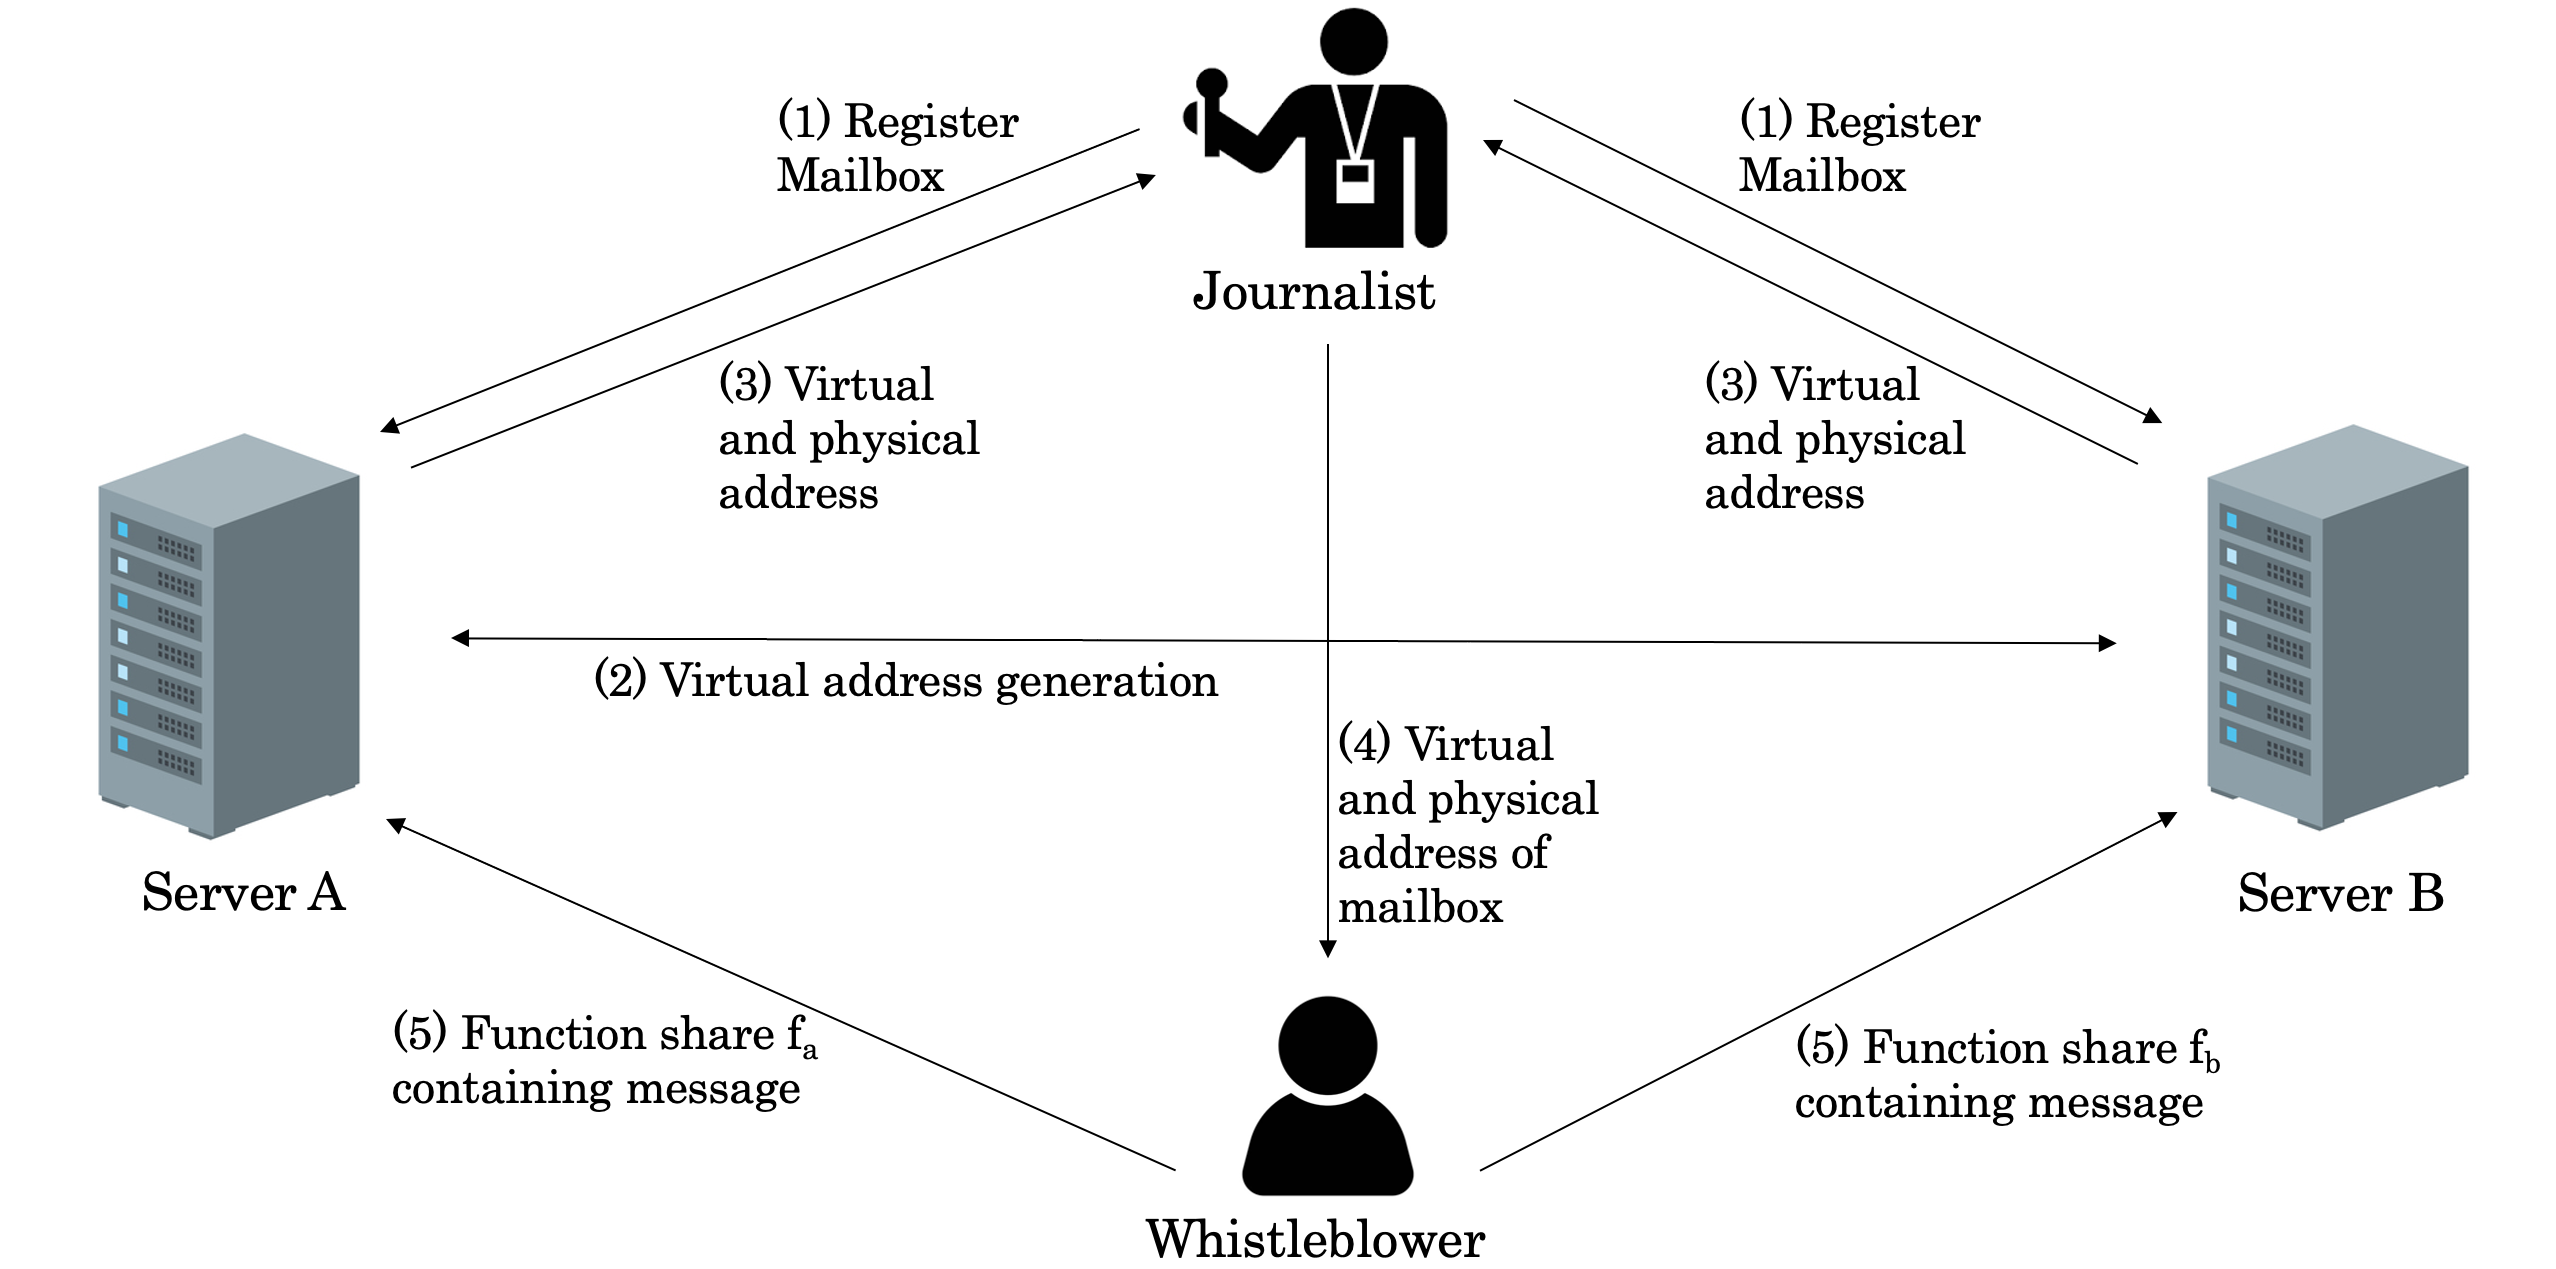
\includegraphics[width= 1\textwidth]{figures/communication.png}
    \caption{Communication between servers and clients. The figure shows the numbered steps from registering a mailbox to sending a message. It does not include the retrieval of a message by a client.}
    \label{communication}
\end{figure}

\subsection{Express Servers} \label{subsec:server}
\textbf{Secret sharing with DPFs.}
Servers A and B together store the entire contents of all mailboxes. Both hold a share of the secret messages, which is implemented using DPFs.
If the express servers hold $n$ mailboxes, each containing an element of the finite field $\mathbb{F}$, the totality of all mailboxes can be represented as the vector $D \in \mathbb{F}^n$. 
$D$ is therefore describing the sum of the two components $D_A+ D_B =D$, where the vector belonging to server A corresponds to $D_A \in \mathbb{F}^n$ and server B's vector corresponds to $D_B \in \mathbb{F}^n$. \\
When a clients sends a new message, they send one share of a vector $w$ containing this message to both servers (further details in section \ref{subsec:clients}). 
Once the servers have received the vectors $w_a$ and $w_b$, they can both add this vector to their current status: \[ D_A \leftarrow D_A + w_A \in \mathbb{F}^n \text{ and equally } D_B \leftarrow D_B + w_B \in \mathbb{F}^n \text{ .}\]This ensures that the received message is placed in the correct mailbox and all other mailboxes remain unchanged. \\
If the servers have a large number of registered mailboxes, they receive vectors with many entries. By using DPFs instead of sending such large vectors, the servers receive only a function share. They can evaluate the function at any point, i.e. for each mailbox. This allows them to recover the vectors $w_a$ and $w_b$ respectively, which they can add to $D_A$ and $D_B$ as before. Section \ref{subsec:DPF} explains in more detail how the functions are created. 
\\ \textbf{Distribution of trust}.
In order to prevent one server from containing all the data, thus representing a single point of failure and not providing adequate security for metadata hiding, multiple servers must be used. One way to achieve this distribution of trust would be to use a large number of servers. This offers the advantage that, even if more than one server is malicious, the system can still continue to run.\\
Express uses only two servers, which in the paper are the ones from Wall Street Journal and the Washington Post. These two servers must therefore meet stricter security requirements. One difficulty in implementing Express could be censorship. If access to one of the two servers is blocked, the entire application will no longer function.  Therefore, Express is less suitable for countries where news websites, i.e. the servers on which Express runs, are often restricted. 
\\ \textbf{Malicious server.}
Another danger is posed by a malicious server. A denial-of-service attack can originate not only from a client, but also from a server. The server can overwrite the contents of all mailboxes with meaningless content, causing the original content to be lost. However, since the client will realise that the contents of their mailbox are garbage, they can recognise that the system can no longer be trusted. 

\subsection{Express Clients} \label{subsec:clients}
\textbf{Write into a mailbox.}
Messages sent by clients should either all be the same size, or they should consist of a predefined set of sizes. If an attacker can extract information from the size of a message, the system will lose security and cover traffic will no longer provide sufficient plausible deniability.
When a client wants to write a message $m \in \mathbb{F}$ into a mailbox, they can insert it into a vector of the length of all mailboxes by multiplying it with the $i$-th standard-basis vector $\mathbf{e}_i$. The value of this vector should be one at the location of the targeted mailbox $i$ and zero everywhere else. Mathematically, this can be formulated as follows: $m \cdot \mathbf{e}_i \in \mathbb{F}^n$. This vector must then be split so that one share can be sent to each server. When these shares are added together, they form the vector containing the message, i.e. $w_A + w_B = m \cdot \mathbf{e}_i$. No relevant information can be obtained from one vector share alone. \\
However, the costs of these calculations are high. Each message sent by the client consists of a vector with length equal to the number of mailboxes in the system. As mentioned in section \ref{subsec:server}, this vector therefore quickly becomes very large, and the fact that both servers receive a vector further increases communication costs.        
A better alternative is to use DPFs, which allows clients to send less data by compressing the vectors $w_a$ and $w_b$. As explained in \ref{subsec:DPF}, it is possible to split a function into two parts that, on their own, do not reveal anything about the function. We call the functions for the two servers A and B $f_A$ and $f_b$. When the functions are added together, they result in the function $f$. $f$ maps indices to function values, i.e. mailboxes to the messages they contain. The function can therefore be evaluated at any point to determine the contents of the corresponding mailbox. This point function can also be written as follows: $f_{i^*,m}: [N] \rightarrow \mathbb{F}$. $i^*$ is the only point at which this function does not output zero, but rather $m$. Clients are able to generate the shares $f_A$ and $f_B$. Added at any point $i \in [N]$, they result in the DPF: \[f_A(i) + f_B(i) = f_{i^*,m}\] Individually, these do not tell an attacker anything about $i^*$, i.e. the mailbox being written to, or about $m$, i.e. the message being transmitted. \\
The use of DPFs has reduced the size of sent messages to such an extent that, with a security parameter $\lambda$, each share of the function now has a length of $O(\lambda log N + \mid m \mid)$ bits. \\
\textbf{Read from a mailbox.} To query the contents of a mailbox, the client sends the physical address $p$ as well as the virtual address of its mailbox to servers A and B. The servers check their page table to see if this is a correct combination of physical and virtual addresses. Then, each of them sends the contents of the corresponding mailbox $D_{Ap}$ and $D_{Bp}$. Afterwards, the servers empty this mailbox by setting the values of $D_{Ap}$ and $D_{Bp}$ to a new encryption of zero with the keys $K_{Ap}$ and $K_{Bp}$. The client uploaded these keys when creating the mailbox. The owner of the mailbox can now use their keys $k_{Ap}$ and $k_{Bp}$ to decrypt the received contents from both servers. They add these decrypted parts of the messages $m_{Ap}$ and $m_{Bp}$ and receive their secret message $m$. 

\section{Protecting Privacy} %auditing, malicious client protection, virtual addressing.
%Explain how these mechanisms maintain security with minimal overhead.
\label{sec:protecting}
The main security requirement that Express must meet is that after an honest client writes a message to a mailbox, an attacker cannot learn anything about which mailbox the client wrote into. 
In this section, we will first demonstrate how Express ensures privacy when all clients behave legitimately, and then when at least one is malicious. Additionally, in the section about the auditing protocol, we will show how security can be provided when not only a client but also one of the servers are malicious. Finally, we demonstrate how Express can be used as a tool for communication between whistleblowers and journalists.  

\subsection{Privacy with honest clients}
The previous chapter \ref{sec:private} explained how we can write a secret message to the server. However, an adversary could now check all network traffic. While they would not be able to read the encrypted message without the keys, they could find out which client wrote to which mailbox by comparing the contents of all mailboxes after each write. \\
To ensure that the metadata is completely hidden, we also need to control who reads the mailboxes. This can be achieved by only allowing reading once all clients have written, i.e. by running the system in batched rounds. Pung and Riposte are based on this concept. However, this severely limits actual usability. Therefore, Express has proposed a method that does not require synchronised rounds. For this, we must ensure that an attacker cannot view the messages or identify which mailbox has been modified after a message has been sent. The only person entitled to this information is the owner of the mailbox. If a mechanism is found that meets these two requirements, a network adversary will still be able to determine when something was written, but will not learn anything about the modified mailbox.\\
To achieve this, Express uses a lightweight cryptographic algorithm based on symmetric cryptography. Servers do not need to authenticate clients when they submit a read request. Before changing the contents of a mailbox, the servers must decrypt all the mailboxes and re-encrypt after the modifications. Both servers have their keys $k_A$ and $k_B$ respectively for each of the mailboxes. The re-encryptions after writing are randomized. This means that an attacker reading the encrypted contents cannot find out which mailbox a new message has been stored in unless they have both keys. \\
A counter is used for encryption. So when re-encryption is required, the previous value is subtracted and the new value added, which is a commutative operation. Re-encryption is only necessary after a read has occurred between writes, not after every write. Otherwise, no information has been obtained by anyone, including an attacker. This increases the efficiency of encryption. Additionally, it is not absolutely necessary for both servers to perform the re-encryption. If one of the servers has been corrupted and no longer re-encrypts, the system remains secure. 

\subsection{Privacy with malicious clients}
The techniques presented in the previous chapter only provide security as long as all clients behave honestly. Even a single malicious client can attack and damage both servers. Nothing prevents a client from creating a vector that writes to multiple mailboxes simultaneously. To do this, it creates a DPF whose added vectors $w_A$ and $w_B$, calculated from the functions $f_A$ and $f_B$, are not equal to zero at multiple inidices. Mailboxes at Express can only hold one message at a time. If a new message is written, the old one can no longer be read. Thus, one message from a malicious client is sufficient to overwrite multiple or even all mailboxes and thereby deleting the original content. To prevent this scenario, Express has introduced an auditing protocol. This protocol ensures that each write update only affects one mailbox. Each vector $w = (w_a + w_b) \in \mathbb{F}^n$ to be inserted must therefore have zero as an element at every position except one. If the vector does not meet this requirement, it can be discarded, meaning the server rejects the write request and nothing is written to any mailbox. \\
Another danger posed by a malicious client is a targeted attack on a specific mailbox. The client, which can no longer write to multiple mailboxes due to the auditing protocol, still has the ability to write a message to a specific mailbox.
We will explain these two concepts in more detail in the following two subchapters. 

\subsubsection{Auditing Protocol}
The auditing protocol must meet three conditions. The first property is completeness: if all parties are honest, the auditing protocol always accepts. In addition, soundness must be fulfilled. If a malicious client submits an invalid write request, the two honest servers must reject it. Finally, the zero-knowledge property must also be met: a malicious server cannot learn anything from a write request from an honest client, except that the request is valid. \\
Express has developed a new auditing protocol that differs from Riposte's previous one in terms of the number of servers required, as well as the computation times and costs. Riposte requires three servers, only one of which may be malicious. The time required for a write in Riposte is linear, which leads to high costs for clients. The auditing protocol developed in Express has a constant runtime, making it much more suitable for real-world applications. In section 5, we will compare the performance of these two systems more detailed. \\
The purpose of the auditing protocol is to verify the Hamming weight of the received vector $w$, i.e. the number of non-zero positions. The message is only valid if this number is one. An n-variant polynomial based on shared randomness between the two servers is used, and no interaction between them is required. If exactly one $w_i$ is non-zero and corresponds to the message $m = w_i$, then the polynomial will most likely result in zero for random choices of $r_1, ..., r_n$: $f(r_1, ..., r_n) = (\sum_{i \in [n]}w_i r_i)^2 - m(\sum_{i \in [n]}w_i r_i^2)$.  This formula checks whether the square of the random linear combination and the sum of the terms of the linear combination squared are equal to each other. 

However, this approach is only secure against semi-honest servers, i.e., servers that follow the protocol but attempt to learn information they should not know. A malicious server, on the other hand, could deviate from the protocol and thereby obtain information about the mailbox to which the client wants to write to by finding the entry $w_i$. To do this, it can modify the received vector and write content to a specific index $i$. If the audit fails and the combined vector $w_A + w_B$ is rejected due to its hamming weight being not equal to one, the server knows that the client from which the vector originated does not want to write to mailbox $i$. If, on the other hand, the message is accepted, the server can be sure that the write request it got is intended to modify the index $i$. \\
To protect against malicious servers, Express performs its auditing protocol within the secret-shared non-interactive proof (SNIP) system \citep{Prio2017}. The exact functionality of SNIP proofs is treated as a black box here and is explained more detailed in the Express appendix \citep{Eskandarian2021}. Each client sends an arithmetic circuit "verify()" in addition to its share of $w$. Servers with only $w_a$ or only $w_b$ can compare with each other whether verify(w)=1. To do this, they need to be able to rely on shared randomness. During the setup phase, servers A and B agree on a shared secret. Using a pseudorandom generator, they can create a new, shared random seed $r$ for each execution of the protocol. The servers first send $r$ to the clients. They then calculate the message shares $m_a$ and $m_b$ by summing up elements in their received vectors $w_a$ and $w_b$, because only one element is non-zero. Additionally, the servers generate several random numbers using their random seed and insert them into a vector $r = (r_1,...,r_n) \in \mathbb{F}^n$. The servers then square each element of this vector to get $R=(r_1^2,...,r_n^2) \in \mathbb{F}^n$. By combining these generated vectors with their received vectors, the servers can create their check values, which represent the inner product between the vectors: $c_A \leftarrow \langle w_A, r \rangle \in \mathbb{F}$, $c_B \leftarrow \langle w_B, r \rangle \in \mathbb{F}$, $C_A \leftarrow \langle w_A, R \rangle \in \mathbb{F}$, $C_B \leftarrow \langle w_B, r \rangle \in \mathbb{F}$. \\
The client must prepare its proof input to convince the server that its input is legitimate. From the server it has received $r$ and the client also knows the index $i^*$ at which it wants to write. It can now derive $r^*$ and $r^{2*}$, which is $r$ at the position of $i^*$, i.e., a secret random number associated with the mailbox being written into. The client then calculates the check values of its two vector shares by multiplication: $c^* = r^* \cdot (w_{Ai^*}+w_{Bi^*})$ and $C^* = r^{*2} \cdot (w_{Ai^*}+w_{Bi^*})$. As the client knows the index $i^*$ of its message, it only needs to perform these calculations for this one entry, giving it a  time complexity of $O(1)$. The servers, on the other hand, have to perform these calculations for all elements, which means they require linear time $O(n)$. \\
The client must now prove that $c^2 -m \cdot C = 0$ where $c \leftarrow c_a + c_B$ and $C \leftarrow C_A + C_B$. To do this, it prepares a SNIP proof $\pi = (\pi _A, \pi _B)$. It sends $\pi _A$ to server A and $\pi _B$ to server B. The servers can then verify the proof together through communication.
The soundness property of the SNIP proof ensures that the servers will only accept a proof if the corresponding statement is valid. At the same time, the zero-knowledge property guarantees that, as long as at least one server behaves honestly, the verification process reveals no additional information about the client's write request, even if the other server acts maliciously.
\\
SNIP proof's computation and communication time are linear in the number of multiplications between secret values. The formula from the auditing protocol only requires two multiplications, two squarings and one multiplication my $m$, the SNIP proof runs in constant time. 
As the performance bottleneck on the server is the evaluation of DPFs, improvements in auditing would not result in significant progress of the overall performance.\\
In the following section \ref{subsubsec:targeted} we will explain that auditing does not protect against attacks on a single mailbox and how we prevent these attacks instead.

\subsubsection{Targeted attacks}
\label{subsubsec:targeted}
An adversary could write random data to a specific mailbox. The recipient can easily tell that their mailbox contains no meaningful information and that the original contents must have been deleted. However, as these messages are sent in a formally correct vector, it is not possible to intercept them using a protocol. \\
To solve this problem, Express uses virtual addresses for its mailboxes. Each mailbox is assigned a 128-bit virtual address. Clients that want to write to a mailbox must know this address. While the physical address space holds approximately $2^{20}$ entries, the address space has a size of $2^{128}$ with 128-bit addresses. This is equal to $3.4 * 10^{38}$, meaning there is such an enormous amount of virtual addresses that most of them are never used and an attacker would never be able to guess a victim's mailbox.  \\
Internally, this is implemented by page tables. Express maintains an array of $n$ physical addresses and an array of $2^\lambda$ virtual addresses, where $\lambda$ is a safety parameter. The servers jointly maintain a page table in which they map the physical addresses to the virtual ones. These tables are stored without encryption on the servers, as their only goal is to prevent attacks by malicious clients. When a client registers a new mailbox, the servers assign it a random virtual address and the corresponding physical address and return these two to the client. Either one server chooses the virtual address itself and communicates it to the other, or both servers determine one together using shared randomness. The servers reserve memory for a new physical address and add this and the created virtual address to the page table. \\
When a client wants to send a message, it creates a DPF with the shares $f_A$ and $f_B: 2^\lambda \rightarrow \mathbb{F}$ as if it were writing to the virtual address space. When creating the message, the client must know both the physical and virtual addresses of its destination mailbox, otherwise its DPF cannot be checked by the auditing protocol. Using its page table, the server can now evaluate the function only at locations where a mailbox actually exists. This prevents the servers from having to perform an exponential number of calculations, which would result in excessively long computation times. 

\section{Express for Whistleblowing}
\label{sec:whistleblowing}
As explained in the previous chapters, Express offers a secure communication option.  In addition to the data transfer itself, two further safety issues should be considered. First, plausible deniability is required; secondly, we need a way to agree on a mailbox address. 

\subsection{Cover traffic}
If Express were only used by whistleblowers, it would be obvious that anyone who sent a message over this application had passed on information. This means that many users that are not involved in whistleblowing must also send messages to create cover traffic. This can be achieved by integrating a JavaScript program into a high-traffic website, such as a news site. Each time a user visits this site, a dummy request is sent to the Express servers. The servers then generate a key that is not known to any client. This means that these messages cannot be read, but they also cannot be distinguished from those of the whistleblowers. \\
The cost and computation times of a dummy request are very low, so these do not pose an issue when integrating Express scripts into the website. The loading times of the New York Times, Washington Post and Wall Street Journal were analysed. They take between 2 and 5.5 seconds to load completely. The Express client in JavaScript needs 51 ms to send 1 KB of data. This means that the calculation times of the client in the browser correspond to less than 3\% of the current loading time. The JavaScript code would only increase the size of these pages by less than 1.5\%. The JavaScript can therefore be executed in the background without affecting the user. \\
News websites like the New York Times benefit from high cover traffic because whistleblowers feel safer and are more likely to pass on information. This makes such sites particularly suitable for integrating the Express code. While Express does not specify exactly how much cover traffic is required, it should be sufficient to ensure that real messages remain indistinguishable from the generated ones.

\subsection{Dialing}
To select a mailbox address, the journalist and the whistleblower can meet in person. However, this is often not possible. In this case, they can use a dialing protocol. For example, the Riposte system could form the basis of a faster, cheaper system incorporating the improvements identified in Express. Journalists can post their public keys for Riposte online and whistleblowers can use this key to send them an encrypted Express mailbox address. Journalists can then download their messages, decrypt them with their private key and register the mailboxes. This approach requires the client to select a virtual address instead of the servers. However, since the address range is so large, it is very unlikely that this address is already in use. 

\section{Related work} %Hier vlt Tabelle mit O notation nehmen und zusätzlich die von Pung und Riposte und vergleichen

% Here, you include short descriptions of similar work and explain \textit{how} they are different from the main content you have presented. Level of detail similar to an abstract. 

\label{sec:relwork}
In this section we will introduce Pung, Riposte and Addra, three cryptographic metadata-hiding communication systems working with the concept of mailboxes. Additionally, we present SecureDrop \citep{securedrop}, a system developed for whistleblowing purposes which has been in use since 2013. Then we will compare their security and performance to Express. SecureDrop, Pung and Riposte were developed prior to Express and were referenced in the paper on Express. Addra, on the other hand, was developed later and uses Express as a source.\\ 
SecureDrop handles the same problem as Express, but takes a different approach to privacy and does not offer cryptographic security. Pung addresses the same problem as Express, focusing on a solution for whistleblowers, but uses more computationally intensive public key cryptography. Addra extends the goal of metadata-hiding even further, presenting a solution for making secure and private voice calls \citep{Ahmad2021}. Riposte uses similar methods to Express, but it hides only the users' identities, not the message content.

\subsection{Pung} 
Pung \citep{Angel2016} is designed to provide privacy guarantees of both message content and metadata. It focuses on protection against powerful global adversaries who may control the entire network infrastructure. This could be mass surveillance or state-sponsored attacks. In Pung, clients deposit and retrieve messages via untrusted key-value stores. Only one server is required. Pung provides privacy even when the server is malicious.  \\
The main goal of Pung is to hide the communication patterns of clients who already know each other's identities. It allows two or more users to exchange messages over a public network without anyone else discovering that they have communicated. To prevent network surveillance, Pung operates in rounds. In each round, a client can only send and receive a limited number of messages. If this limit is exceeded, users must wait for the next round. Message retrieval is based on private information retrieval (PIR). This is a protocol that allows clients to send a request to a database without the server on which it runs knowing which items were fetched. This protocol is expensive and as a result, clients should download large amounts of data simultaneously to improve its performance. Pung is therefore particularly suitable for applications where this is the case, such as emails or group chats. Otherwise, the cost of network traffic is relatively high.\\
While significantly reducing the costs compared to prior approaches, Pung's network costs remain high. However, newly introduced techniques have significantly reduced the cost of cryptographic calculations.


\subsection{Riposte}
Riposte protects against network surveillance and malicious clients \citep{Corrigan_Gibbs_2015}. Like Express, its main target group is whistleblowers who want to leak information anonymously. Riposte users can post messages anonymously on a bulletin board, which acts as a public broadcast channel. Clients have a fixed time window in which they can write their messages. These messages are collected on the server and published when the time window has expired. At this point, everyone can read all the previously written messages. The content is therefore not secret, but the author remains anonymous. If messages were published after each write, it would be possible to see who was last connected to the server and therefore who created that message.\\
Riposte can be used in two ways. Either with three servers, only one of which may be malicious, or with a variable number, at least one of which must be honest. The variant with three servers, at least two of which are honest, uses a less expensive protocol. This is preferable when millions of clients use Riposte, and is also the variant compared with Express in the paper. \\
Riposte's key innovation was to minimise the amount of data each client uploads to the servers by using DPFs and a private information retrieval (PIR). This makes large-scale anonymous writing more practical than with earlier systems. However, it relies on public-key cryptography and synchronized communication rounds, which still lead to computational and communication overhead.


\subsection{SecureDrop}
SecureDrop \citep{securedrop} is an open-source whistleblowing platform \citep{berret2016guide}. It is used by news organizations to enable anonymous, secure exchange of documents and messages between sources and journalists. Maintained by the Freedom of the Press Foundation, it is deployed by numerous media organizations worldwide, including The New York Times and The Guardian. SecureDrop was originally developed by Aaron Swartz, an activist against internet censorship, and Kevin Poulsen, who was earlier pursued by the FBI and spent five years in prison for computer fraud. SecureDrop aims at protecting the identity of whistleblowers and the confidentiality of leaked information. Sources submit documents and messages through the Tor network, which hides the network location and identity of sources from both the news organisation and potential adversaries. The system stores encrypted submissions on servers that are physically secure and disconnected from the wider organisation's network. Journalists access these servers through separate, hardened machines that are kept offline to prevent data leaks.
While SecureDrop provides strong confidentiality of content and reasonable anonymity at the network level, it does not achieve cryptographic metadata privacy. An adversary who monitors a large portion of the network, especially the Tor network used, might still detect that a communication occurred \citep{securedropTraffic}.


\subsection{Addra}
Addra is dedicated to hiding metadata during voice calls \citep{Ahmad2021}. This data, which includes information such as call duration, time and parties involved, is highly sensitive and of great interest to government surveillance programs. Addra is the first system to hide metadata from voice communications over a completely untrusted infrastructure. Previous systems with the same objective were either not sufficiently scalable, supporting a maximum of a few dozen users, or they required trusted partners, which posed a security risk. \\
Callers receive a mailbox when they initiate a call, regardless of who the call is going to. They place their message in it to prevent an enemy from finding out who the call is going to. Using the PIR protocol, the callee can retrieve the message from the mailbox. 
Addra extends Pung's protocol by using public and private keys to establish secure communication channels. Addra uses Pung's PIR protocol with private and public key encryption. However, Addra has expanded it to FastPIR. This reduces calculation times on the server side. In addition, PIR calculations are parallelised, as low latency is essential for calls. \\
Addra has demonstrated that, in addition to sending messages, metadata privacy is also important in more demanding areas and can be implemented using similar methods. 


\subsection{Comparison}
All five applications focus on combining scalability with strong privacy guarantees against network surveillance and malicious servers. A significant limitation of Pung and Riposte compared to Express is that both operate using batched rounds, meaning each client must have written their message before anyone can read it. This simplifies anonymity guarantees but restricts usability, since communication can only proceed once all clients in a round have acted. Batch processing introduces high latency, making real-time interaction impractical. Express eliminates this limitation with an asynchronous architecture that allows clients to write and read messages independently. This improves responsiveness and reduces the coordination overhead that previously limited scalability. Therefore, Express offers comparable cryptographic privacy alongside a better user experience. \\
Riposte focuses on anonymous public posting, functioning as a broadcast channel rather than a private messaging service. Pung and Addra on the other hand enable private message exchange between known parties over an untrusted infrastructure. However, both systems achieve this by accepting higher computational and network costs, which limits their scalability to smaller user groups. \\
SecureDrop works most differently compared to the other four applications. It is vulnerable to traffic analysis if a large proportion of the network is monitored. As metadata is not fully  cryptographically hidden, an adversary could still detect that communication occurred between a whistleblower and a journalist, even if they cannot read the content of the messages. Furthermore, maintaining SecureDrop requires a trusted infrastructure within the media organisation, including physical security for the servers and trained operational staff.

In an era of ever-expanding technical possibilities and heightened interest in metadata among nation-states, relying on trusted servers is risky. These servers can be attacked by states using their enormous political and financial resources. This is why Pung and Addra, which continue to operate without a trusted infrastructure, offer the strongest security. Riposte and Express take a different approach by distributing trust across two or more servers. Compared to Riposte, Express strengthens its security guarantees through an auditing mechanism that detects malformed client requests and prevents data corruption without revealing metadata.
This protection against malicious clients makes Express more robust in practical deployments while still maintaining a realistic trust model. Therefore, Express provides a balanced compromise between strong cryptographic privacy and operational practicality, making it more suitable for large-scale or real-world use.

\subsubsection{Performance}
Significant events prior to Express's research led to it testing larger messages than previous systems. In 2019, a whistleblower submitted a report concerning President Trump's interactions with the leader of Ukraine \citep{WhistleblowerComplaint}. The file had a size of 25.3 KB and demonstrated how important it is to offer whistleblowers the option of sending large messages.

Overall, Express reduces the cost of maintaining a service for whistleblowers by 6$\times$ compared to previous work with the same objective.
In Express, communication costs were compared to those of Riposte and Pung. To do this, \citet{Eskandarian2021} set up three Google Cloud instances, two running the servers and one simluating the clients. Each of them has a 16-core intel Xeon processor with 64 GB of RAM. All three instances ran on the same data center to minimise latency. They were used to evaluate Express, Pung and Riposte (See Table \ref{tab:communication}). The table shows that providing security with only one server leads to high costs. It demonstrates that Express's DPFs and improved auditing protocol have a positive impact on communication costs.
\begin{table}[h!]
\centering
\caption{Communication cost for 1 million mailboxes}
\label{tab:communication}
\begin{tabular}{llll}
\hline
 & Express & Riposte & Pung \\ \hline
Servers needed                             & 3       & 1     & 2       \\ \hline
Client side                                & x       & 101$\times$x & 4631$\times$x  \\ \hline
Server site                                & y       & 195$\times$x & 7161$\times$y  \\ \hline
\end{tabular}
\end{table}

Since both Express and Riposte have multiple servers, these two applications need an auditing protocol. For a fixed security parameter $\lambda$, the auditing protocol used by Express requires $O(\lambda)$ communication between parties. Client-side communication takes a constant time of $O(1)$ with less than 5 microseconds. Riposte, on the other hand, requires communication of order $\Omega (\lambda \sqrt{n})$ and client computation of order $\Omega (\sqrt{n})$. 

\begin{table}[h!]
\centering
\caption{Express vs Riposte performance}
\label{tab:riposte}
\begin{tabular}{lll}
\hline
                           & Express & Riposte   \\ \hline
Auditing protocol compute costs          & x       & 8$\times$x       \\ \hline
Throughput                 & y       & 1.4-6.3$\times$y \\ \hline
Cost of processing 1 million messages & z       & 5.9$\times$z     \\ \hline
\end{tabular}
\end{table}
Table \ref{tab:riposte} shows that Express achieved improvements in runtime compared to Riposte across all operations. It is noticeable that Express not only has a faster auditing protocol, but also has a higher throughput. 
Express's latency, i.e., the time from when a message is sent until it can be read, consists only of the time required to evaluate a DPF write and run the audit, otherwise, no synchronization between client and servers is necessary. In the same time that Express can process 32 KB, Riposte only manages to process approximately one KB, measured with approximately 50,000 mailboxes. Pung is also slower than Express. The difference is particularly noticeable with small messages. With messages of 10KB, Pung is still about 1.3-2.6$\times$ slower than Express, and with 32KB they are approximately the same speed. 
\subsubsection{Cost analysis} In their cost analysis, the authors limited themselves to the cloud infrastructure, so engineers are not included. The biggest cost factor is server operation. Public Google Cloud Platform pricing information can be used to determine the cost in dollars of sending one million messages. This consists of the cost of hosting the servers for the time required to process the messages, plus the cost of the data passed between the servers and the clients. Express costs for one million messages 5.9$\times$ less than Riposte. Pung is again significantly more expensive than Riposte. Sending one million messages costs over \$1,000 with Pung, despite it only operating one server. The main costs are for data egress. Express requires significantly less money for the same number of messages, namely only \$0.05 and Riposte \$2.41.  Since Express only has to maintain two servers rather than three, as Riposte does, it is relatively cheaper per hour.


\section{Conclusion}
\label{sec:conclusion}
We have shown that Express represents a significant advancement in the performance and reproducibility of privacy-enhancing technologies. Its auditing protocol and virtual addressing enable efficient, scalable metadata privacy suitable for use cases such as whistleblowing, investigative journalism, or any communication scenario where metadata leakage poses a critical risk. \\
By comparing Express with the related systems Pung, Riposte and Addra, we demonstrated that Express achieves lower communication and computation costs without sacrificing its privacy guarantees. Unlike systems that trade efficiency for stronger anonymity or that degrade over time, Express maintains robust security properties with practical performance for large-scale deployment. 
Nevertheless, Express still faces challenges common to metadata-private systems, such as the need for at least one honest server. Future work could explore reducing these trust assumptions or extending the protocol to support real-time communication scenarios similar to Addra. \\
Overall, Express contributes an important step toward making metadata-hiding messaging systems fast, secure, reproducible and therefore suitable for real-world communication. 
%particularly suitable for high-volume, privacy-sensitive applications like whistleblower communication systems.

\section{Use of generative digital tools}
%The use of AI tools must always be declared completely and transparently. 
%For examples of how to do this, please see the DMI guidance: \url{https://dmi.unibas.ch/fileadmin/user_upload/dmi/Studium/Computer_Science/Diverses/Wegleitungen/Dokumente_2023/Guidance_on_AI_in_teaching_in_Computer_Science.pdf}.
I used DeepL to translate some sections in my paper that I didn't fully understand in english into german, and to translate individual sentences that I couldn't formulate in english.


\bibliographystyle{apalike}

\bibliography{references}



\includegraphics[width=\textwidth]{wissensch_Redlichkeit_E_09-2023}

\end{document}

how to cite: This sentence is supported by a reference \citep{chaum1981untraceable}.
This sentence is justified with multiple references \citep{chaum1981untraceable,shamir1979how}.
\citet{alley2018craft} as well as \citet{strunk1999elements} use in-line references.


Bild einfügen: \begin{figure}
    \centering
    
\includegraphics[width= 0.3\textwidth]{figures/privacy-screen}
    \caption{An example privacy mechanism}
    \label{fig-privacy-screen}
\end{figure}
Bild zitieren: (See Figure~\ref{fig-privacy-screen}.)


Theorem einfügen: \begin{theorem}[Incompleteness theorem, \citeauthor{godel1931formal}, \citeyear{godel1931formal}]~\\
    If $c$ be a given recursive, consistent class of formulae, then the
    propositional formula which states that $c$ is consistent is not
    $c$-provable; in particular, the consistency of $P$ is unprovable in $P$, it
    being assumed that $P$ is consistent.
\end{theorem}

Tabelle einfügen: (See Table~\ref{tab:example}.)

\begin{table}
	\centering
	\begin{tabular}{p{3cm}ll}
		\toprule
		Header line & Column 2 & Column 3 \\
		\midrule
		Content line & 2 & 3 \\
		Another content line to showcase wrapping of table cells & 2 & 3 \\
		\bottomrule
	\end{tabular}
\caption{An example table}
\label{tab:example}
\end{table}


Ref zu einer Section: Note that you may include the related work as a subsection in the Background Section~\ref{sec:background}. 



The former General Counsel of NSA, Stewart Baker, has said, “metadata absolutely tells you everything about somebody’s life. If you have enough metadata, you don’t really need content”  D. Cole. We kill people based on metadata. The New
York Review, May 2014.